%!TeX root = ../main.tex
\chapter{Doc of the doc}
\label{autodoc}

This chapter expains how this document structure works.
It's aimed at people who (like me) don't know much about \LaTeX.

\section{Basic composing}

Here's what you need to know to create chapters, sections, etc.

You have different levels in \LaTeX to generate different title structures. Here's how it works (but for additional information, check \url{https://en.wikibooks.org/wiki/LaTeX/Document_Structure}).

\begin{lstlisting}[style=Latex-color]
\chapter{This is a chapter}
A chapter starts on a blank page.
Use chapter* in your forewords to exclude them for table of contents.
\section{Big title}
Usually this is what we call level-2 title.
\subsection{Subsection}
This is a subsection content
\subsubsection{Subsubsección}
Guess what it is?
\paragraph{A very deep level}
Here's the paragraph content. See how its content starts on the same line as the title.
\end{lstlisting}
This is how it looks:
    \section{Big title}
    Usually this is what we call level-2 title.
    \subsection{Subsection}
    This is a subsection content
    \subsubsection{Subsubsección}
    Guess what it is?
    \paragraph{A very deep level}
    Here's the paragraph content. See how its content starts on the same line as the title.

Apart from that, linebreaks are ignored. To separate paragraphs, use a blank line.

For example, this is a new paragraph.


This is a new paragraph on a separated blank line.

\section{Footnotes}

\section{Glossary}

\section{Fancy stuff}

\subsection{Images}

Put your images in the \texttt{assets} directory. Then use the following code:

\begin{lstlisting}[style=Latex-color]
\begin{figure}
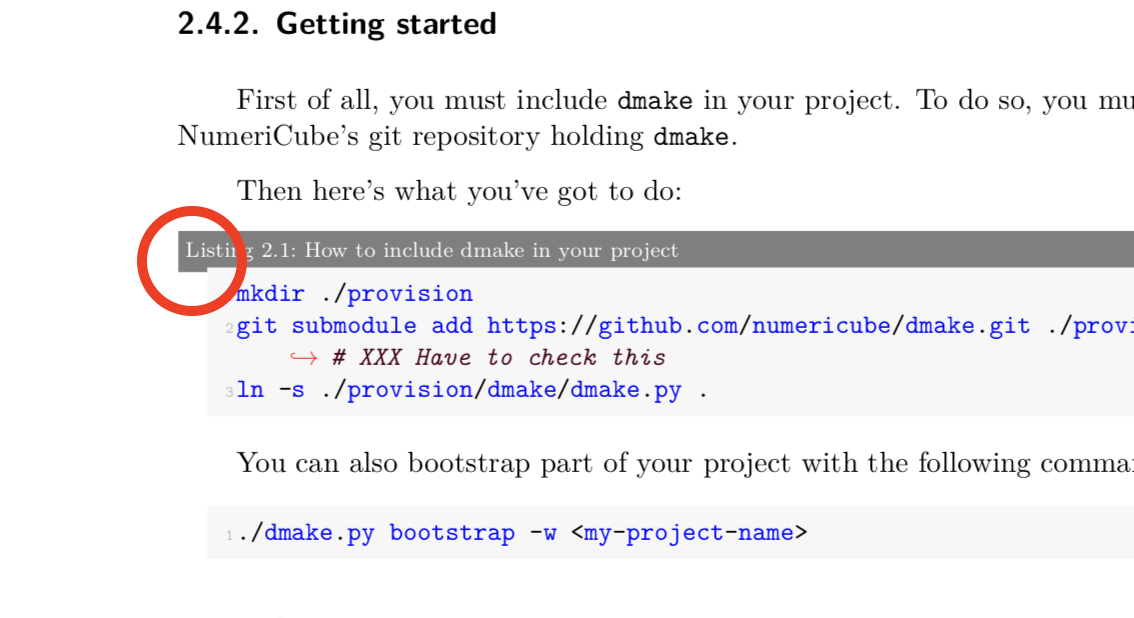
\includegraphics[width=\textwidth]{assets/alignmentpb.png}
\caption{Alignment problem}
\end{figure}
\end{lstlisting}

\subsection{Pretty boxes}

You can include pretty boxes with the \texttt{\textbackslash warningbox} directive.

\begin{lstlisting}[style=Latex-color]
\warningbox{This is a warning box.}
\end{lstlisting}

\warningbox{This is a warning box.}

\subsection{CSV files}

This is how to add a big CSV file.

For the record, this was generated with \texttt{git log \-\-date=local \-\-pretty=format:"\%h\%x09\%an\%x09\%ai\%x09\%s"}

\csvautolongtable[
    separator=tab,
    % no head,
    respect all
]{assets/commits.csv}
% {1=\hash,2=\author,3=\date,4=\comment}
% {\hash & \author & \date & \comment}

\section{TODO}

This is a list of work to be done in the following template.

\subsection{Miscellaneous stuff}

\begin{itemize}
    \item Change BW page to something like this \url{https://www.latextemplates.com/templates/books/2/book_2.pdf} (look at page 3)
    \item Add a backcover page (even if it's just white)
    \item Mention the excellent base template in acknoledgements: \url{https://github.com/jmrplens/TFG-TFM_EPS}
\end{itemize}

\subsection{Caption alignment error}

There's a slight alignment error with code captions when using \texttt{lstlisting} (see screenshot below). It has to be fixed.

\begin{figure}
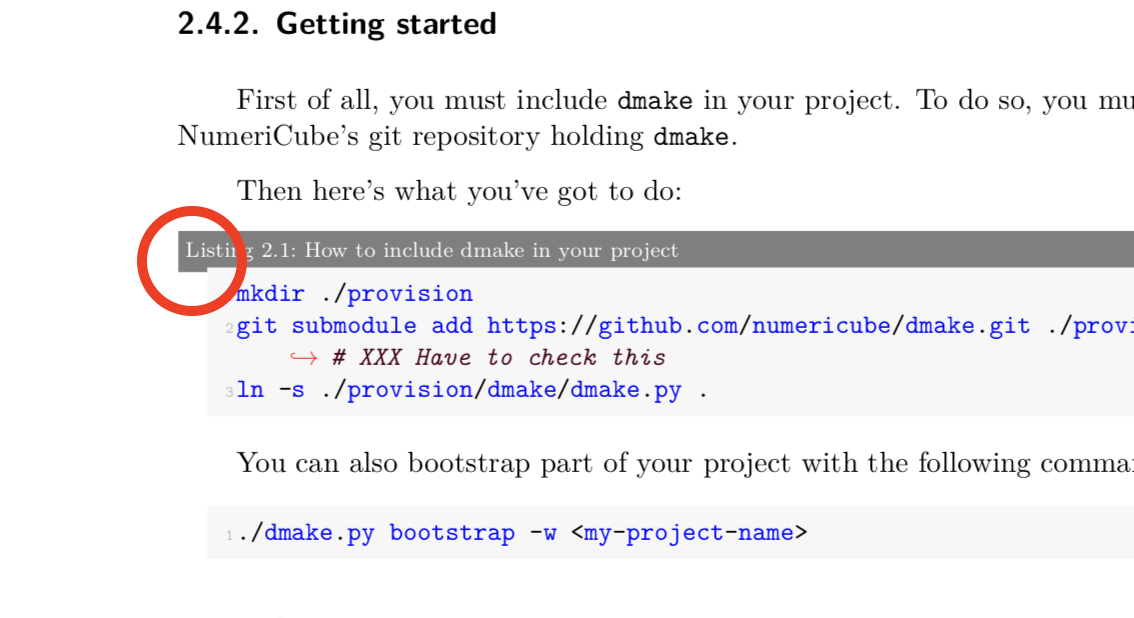
\includegraphics[width=\textwidth]{assets/alignmentpb.png}
\caption{Alignment problem}
\end{figure}


\subsection{Logos}

Logo management is far from perfect, especially on the front page (oops).

Probably need someone to make PDF-compliant EPS versions of my logo in various versions. See table \ref{table:logoformats} on page \pageref{table:logoformats} for a complete list of what we need.

\begin{table}[ht]
	\centering
	% {\scalefont{0.9}
	\begin{tabular}{@{}lccc@{}}
	\toprule
        Filename                        &   Baseline Language   &   Shape   & Base color \\ \midrule
        LogoN3-2018-EN-rect-white       &   English             & Rectangle & White/Transparent \\
        LogoN3-2018-FR-rect-white       &   French              & Rectangle & White/Transparent \\
        LogoN3-2018-EN-square-white     &   French              & Square    & White/Transparent \\
        LogoN3-2018-FR-square-white     &   French              & Square    & White/Transparent \\
        LogoN3-2018-EN-rect-black       &   English             & Rectangle & Black/Transparent \\
        LogoN3-2018-FR-rect-black       &   French              & Rectangle & Black/Transparent \\
        LogoN3-2018-EN-square-black     &   French              & Square    & Black/Transparent \\
        LogoN3-2018-FR-square-black     &   French              & Square    & Black/Transparent \\ \bottomrule
	\end{tabular}
	% }
	\caption{Different types of logos to have in the \texttt{include/logos} folder.}
	\label{table:logoformats}
\end{table}

\subsection{.gitignore}

We should document what should be in \texttt{.gitignore} (and not into git, then).

Ideas comming in mind:

\begin{itemize}
    \item \texttt{docgen} folder
    \item \texttt{build} folders
    \item \texttt{provision/history} folder (or maybe not?)
    \item \texttt{DS\_Store} Mac Finder folders
\end{itemize}

\section{Lorem ipsum (just to check text structure)}

\lipsum

Nous répertorions ici les préreqis nécessaire a l'execution du projet sur l'ordinateur.

\begin{description}
    \item[Bash]: Une fenêtre shell.
    \item[\gls{docker}]: Ceci est utilisé pour lancer des microservices sur votre machine locale.
        Obligatoire pour l'exécution
        Téléchargez le depuis \url{https://www.docker.com}
    \item[Docker compose]: Utilisé pour gérer plusieurs conteneurs à la fois.
        Téléchargez le depuis \url{https://www.docker.com}
    \item[Amazon|Azure \gls{cli}]: Téléchargez et installez la dernière interface de ligne de commande
        Azure ou AWS afin de pouvoir y déployer vos projets.
\end{description}

\section{Dmake, script de gestion Docker}

\texttt{dmake}\footnotemark est le principal point d’entrée pour les projets gérés par Docker + Swarm.
\footnotetext{Permet de monter le Docker}

\subsection{Deployment workflow}

Cette partie explique le fonctionnement du \texttt{dmake}
et \gls{n3} déploiement automatique.


\subsection{Pour commencer}

Tout d’abord, vous devez inclure \texttt{dmake} dans votre projet.
Pour ce faire, vous devez avoir accès au dépôt git de NumeriCube contenant \texttt{dmake}.

Voici les étapes a suivre :
\begin{lstlisting}[style=bash,caption={How to include dmake in your project}]
mkdir ./provision
git submodule add https://github.com/numericube/dmake.git ./provision/dmake # XXX Have to check this
ln -s ./provision/dmake/dmake.py .
\end{lstlisting}

You can also bootstrap part of your project with the following command:
\begin{lstlisting}[style=bash]
./dmake.py bootstrap -w <my-project-name>
\end{lstlisting}

\warningbox{When you include a submodule this way, other users of your main github project
will probably find an empty \texttt{provision/dmake} folder when they clone your project.
In order to avoid that, advise them (ie. put this in your \texttt{README} file) to do the following
after they cloned the project.}

\begin{lstlisting}[style=bash]
git submodule init
git submodule update
\end{lstlisting}

Wait for the day I'll publish it on pip and issue: \texttt{pip install dmake}\footnote{Don't push your luck
too far, I'm too busy right now to do so.}.

\subsection{Basic commands}

See the general philosophy section above to understand how it is working.

\subsubsection{Release}
